%!TEX root = ../main.tex

\newpage
\section*{Supplementary}

  \hl{Copy paste table here once done}

  \renewcommand{\thefigure}{S\arabic{figure}}
  \setcounter{figure}{0}

  \begin{figure}[h]
  \centering
  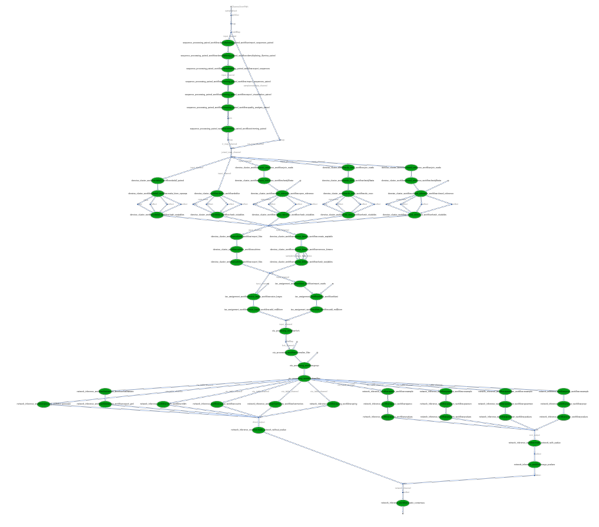
\includegraphics[width=\linewidth]{figureS1.pdf}
  \caption{
    \textbf{Comparison of various denoising and clustering algorithms used in the pipeline}.
    (A, B) Correlation ofjk the abundances of the taxa that are in common between the count matrices created by two different methods.
    (A) The best correlation (most similar methods) is between open-reference and denovo.
    (B) The worst correlation (least similar methods) is between open-reference and dada2.
    (C) A heatmap showing the $\mathrm{R}^2$ of all pairwise comparisons of the methods.
  }
  \label{fig:figureS1}
\end{figure}

  \begin{figure}[h]
    \centering
    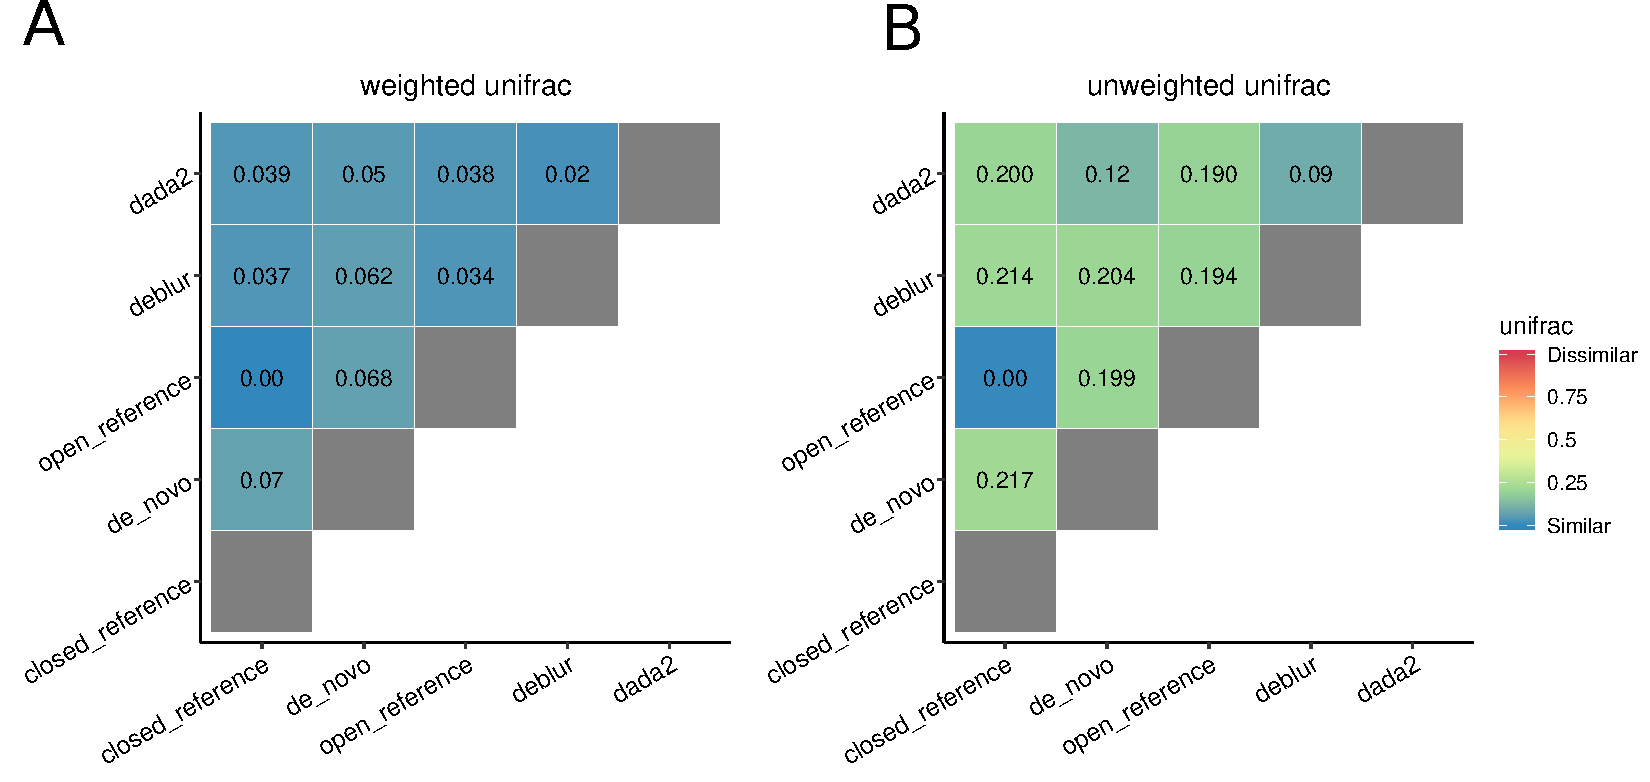
\includegraphics[width=\linewidth]{figureS2.pdf}
    \caption{
      \textbf{Heatmaps showing the weighted and unweighted unifrac distances for the hard palate dataset analysis}.
      (A) weighted unifrac distances and (B) unweighted unifrac distances between the representative sequences generated by different denoising and clustering algorithms.
      These results are in agreement with the stool microbiome dataset.
    }
    \label{fig:figureS2}
  \end{figure}

  \begin{figure}[h]
    \centering
    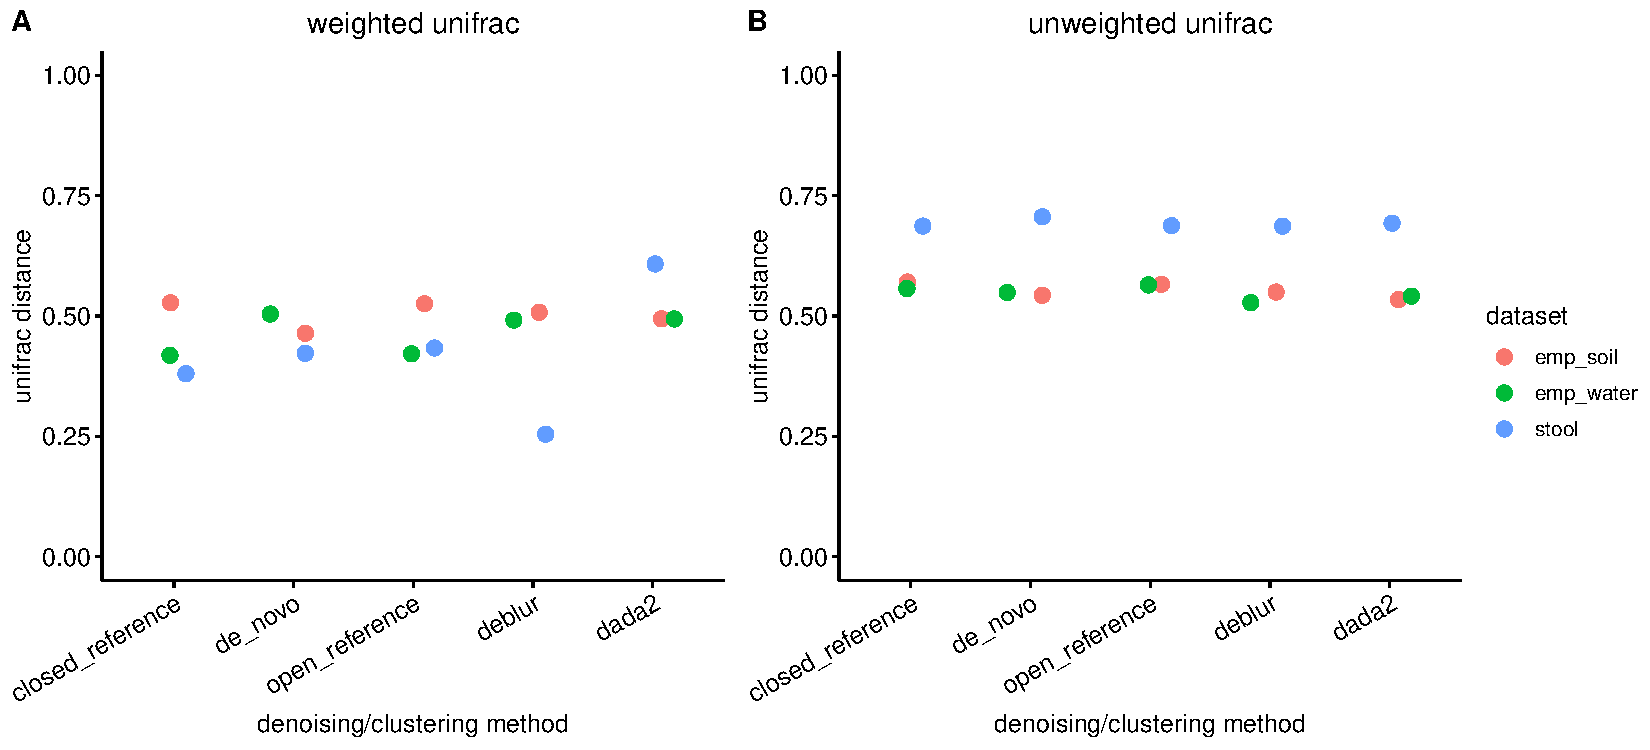
\includegraphics[width=\linewidth]{figureS3.pdf}
    \caption{
      \textbf{The distributions of the average weighted UniFrac distance between the expected sequence profile and the calculated sequence profile in the synthetic datasets}.
      We observe no significant difference between the various methods on the synthetic datasets used for this study.
    }
    \label{fig:figureS3}
  \end{figure}

%   \begin{figure}[h]
%     \centering
%     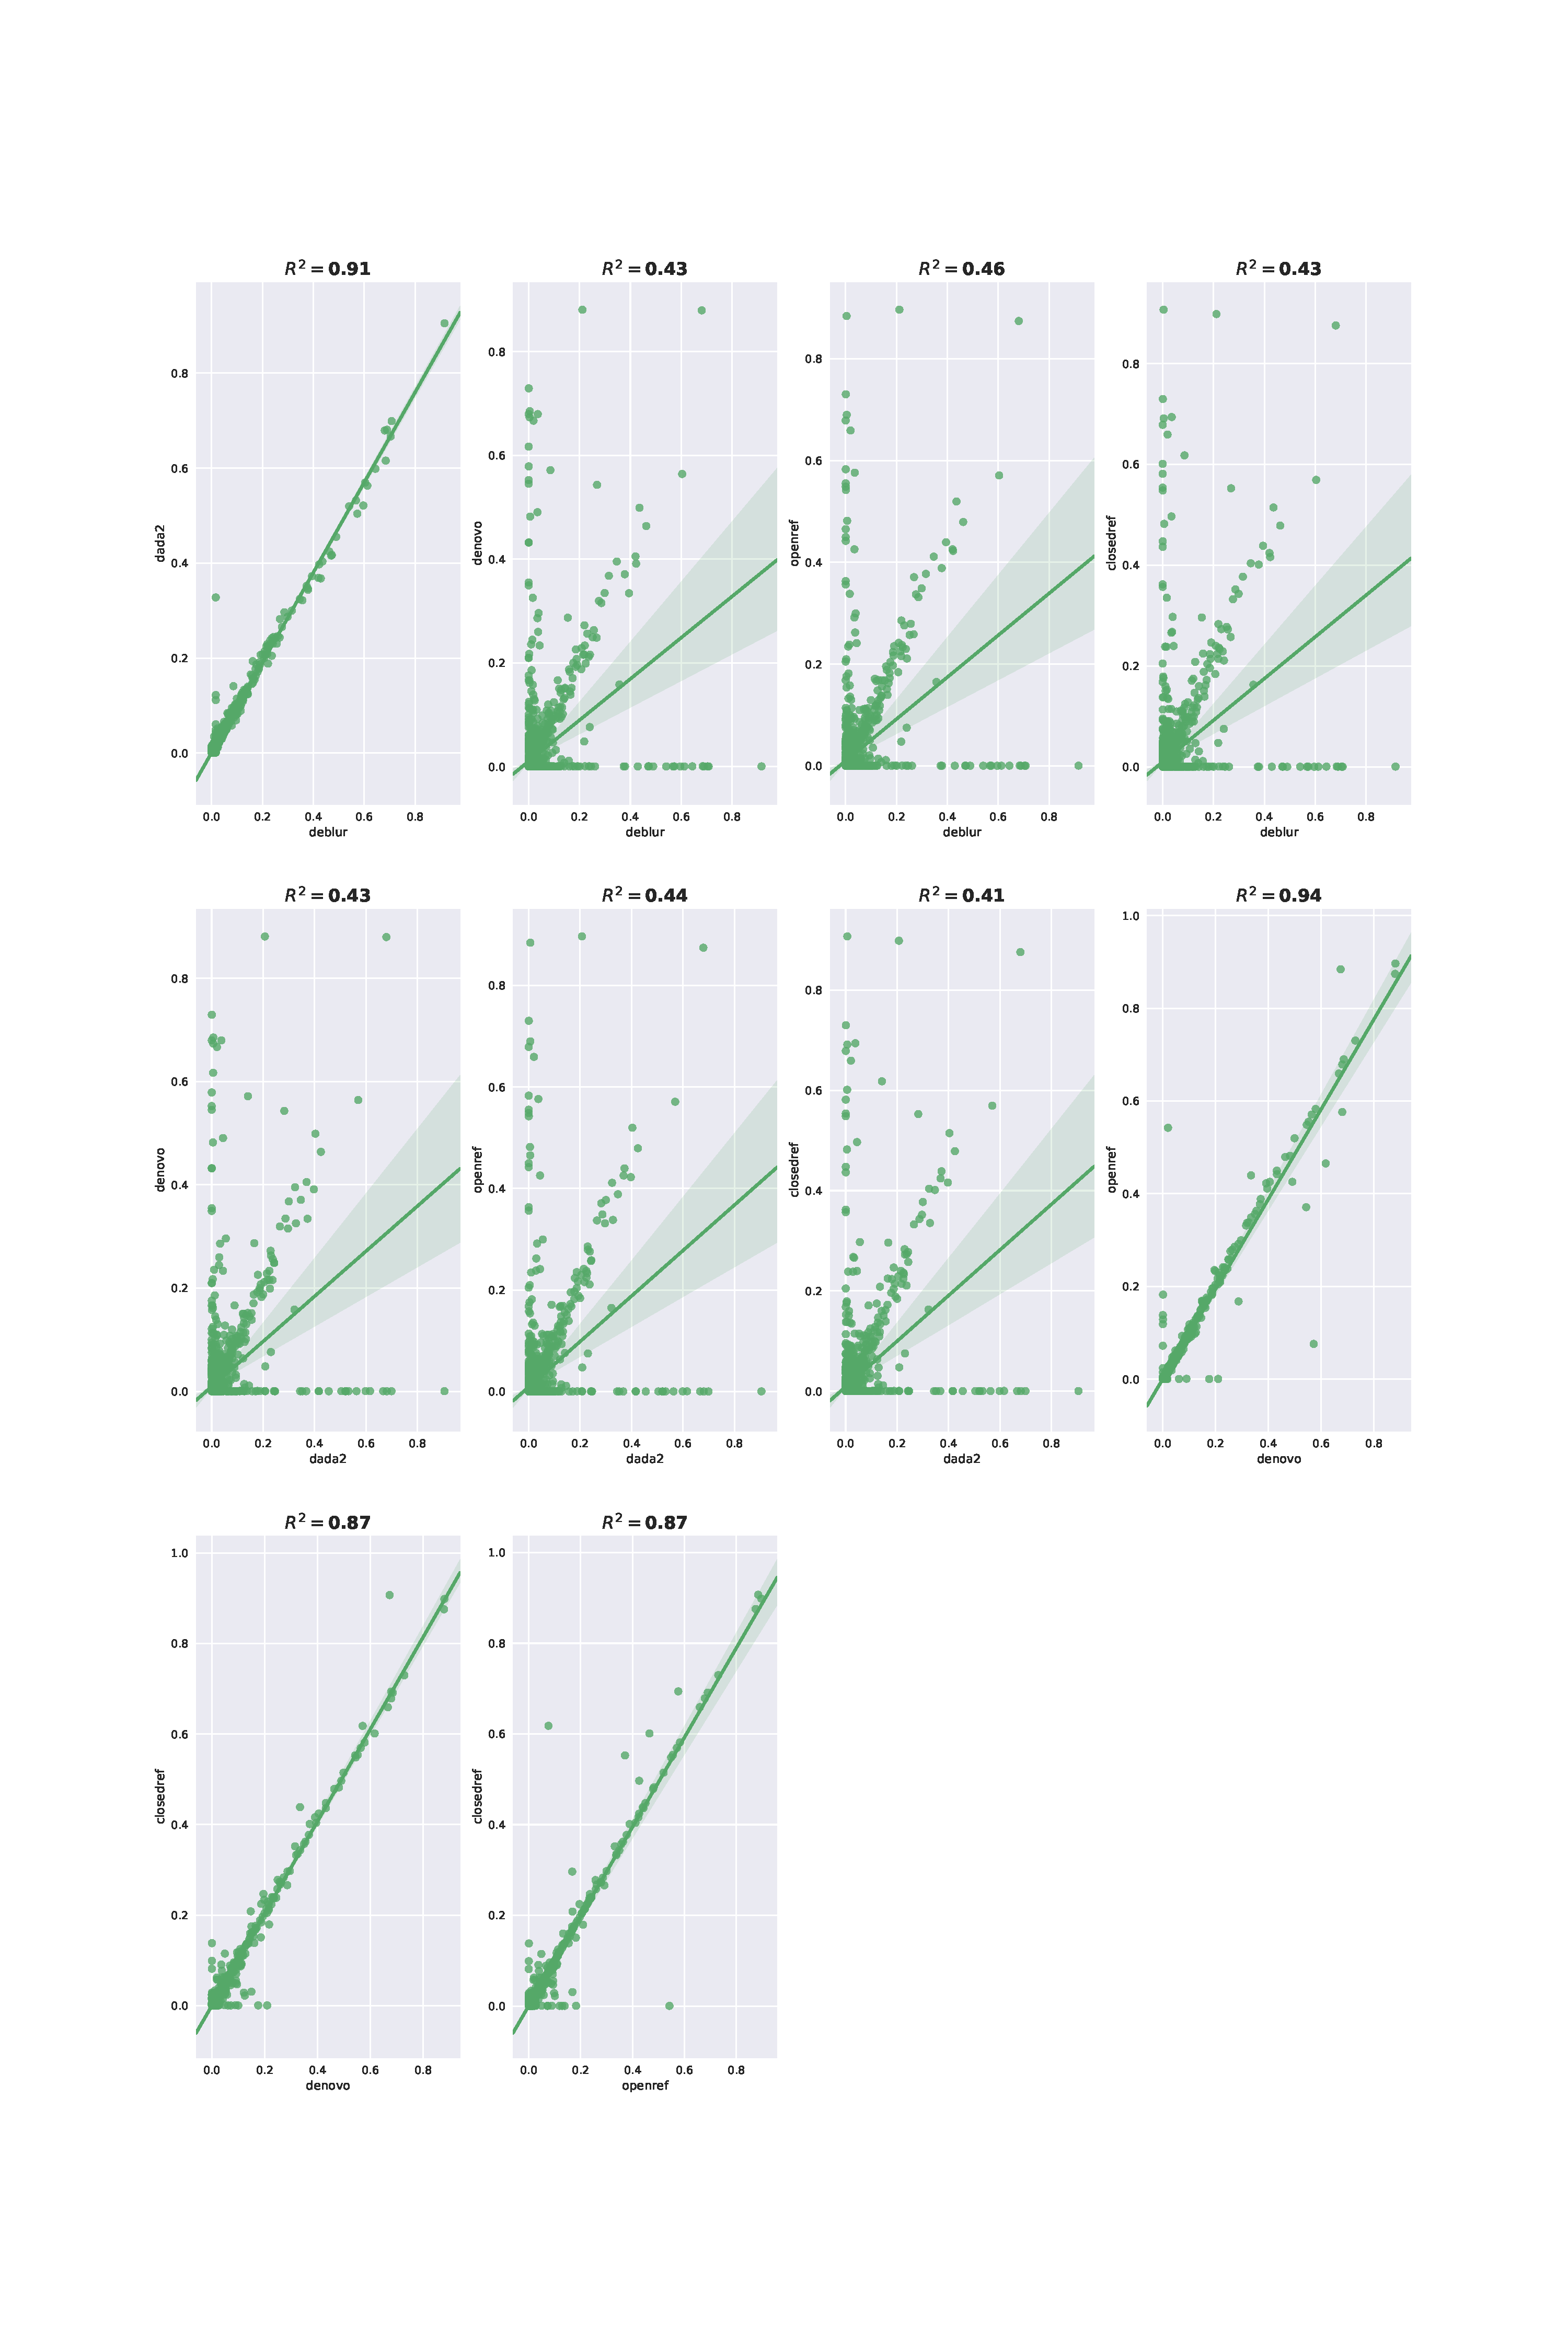
\includegraphics[width=0.9\linewidth]{pdf/all_denoise_reg.pdf}
%     \caption*{All pairwise correlations comparing the similarity between different denoising and clustering methods}
%     \label{fig:figureS4}
%   \end{figure}

  \begin{figure}[h]
    \centering
    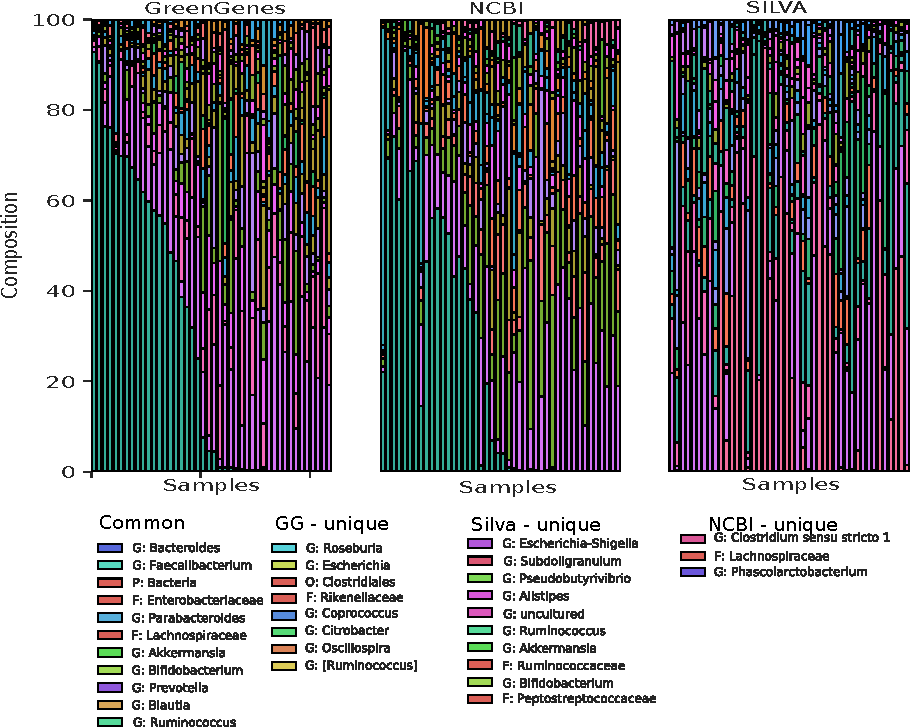
\includegraphics[width=\linewidth]{figureS4.pdf}
    \caption{
      \textbf{(A)} Taxonomy composition of the 20 most abundant genera predicted for the stool microbiome dataset generated using different taxonomy references databases: Greengenes, SILVA and NCBI.
      The legend shows the common and the unique genera among the taxonomy assignments.
  }
    \label{fig:figureS4}
  \end{figure}

  \begin{figure}[h]
    \centering
    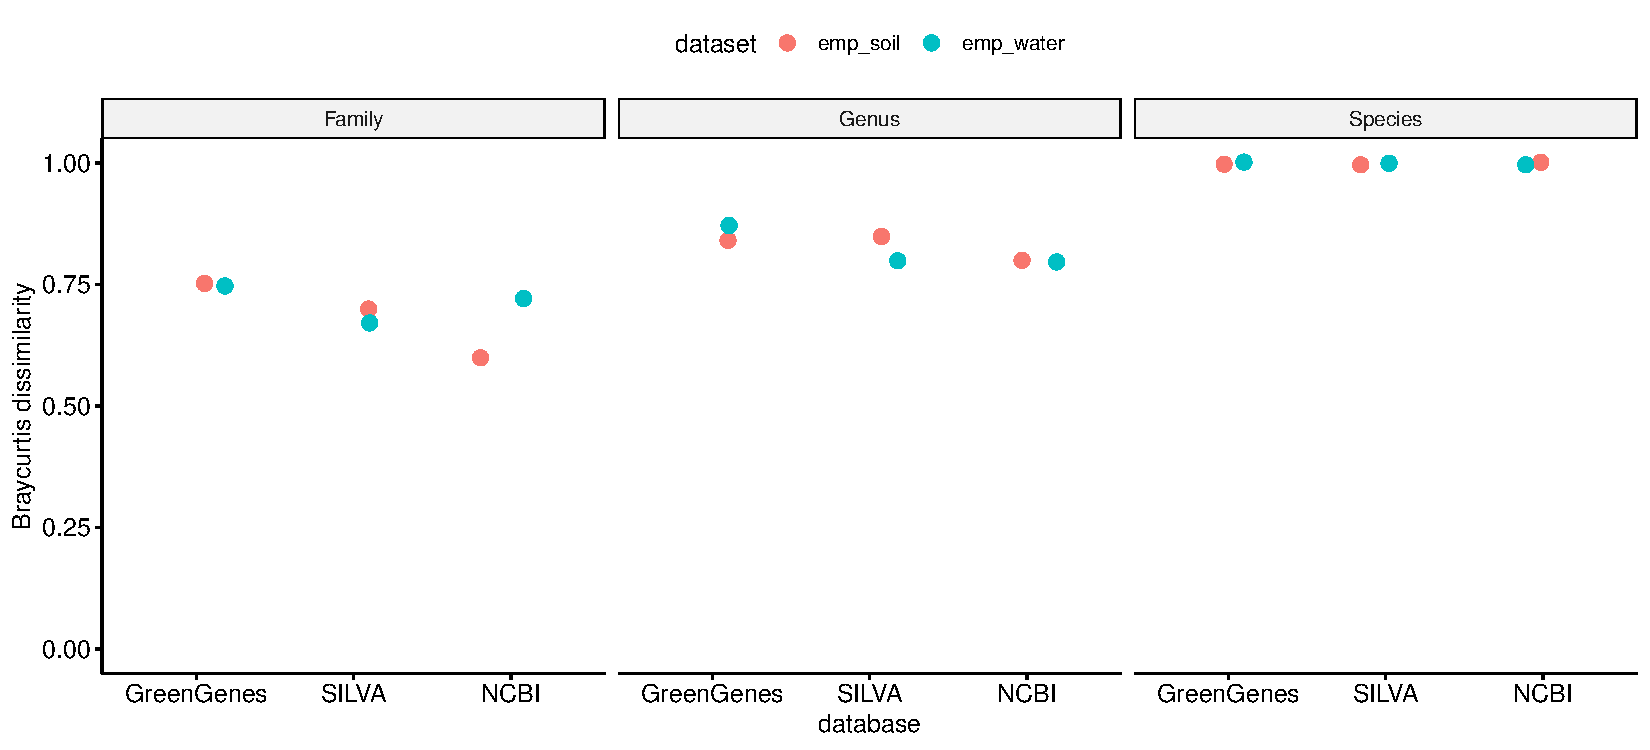
\includegraphics[width=\linewidth]{figureS5.pdf}
    \caption{
      The bray-curtis dissmilarity between the expected taxonomic composition and generated taxonomic composiion for the synthetic datasets.
  }
  \label{fig:figureS5}
  \end{figure}

  \begin{figure}[h]
    \centering
    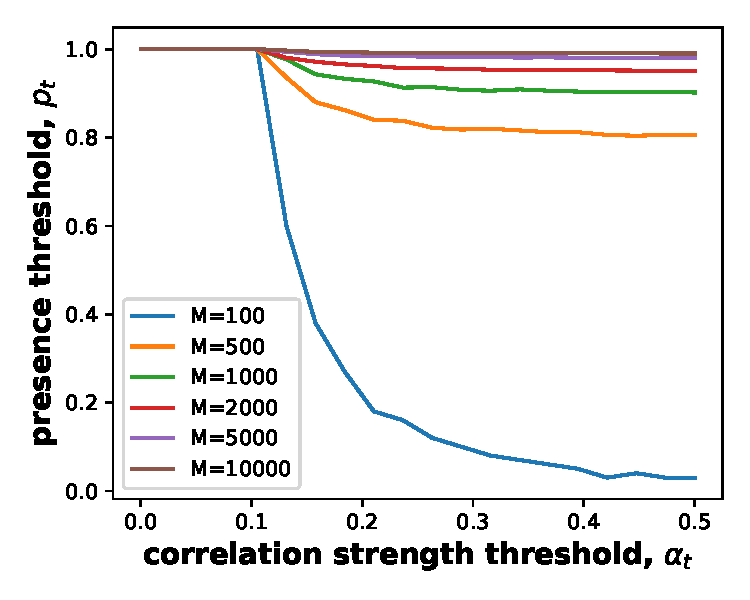
\includegraphics[width=\linewidth]{figureS6.pdf}
    \caption{
      Calculation of presence threshold that is applied on the OTU table in the OTU processing (OP) step of the pipeline.
      This presence threhold $p_t$ is dependent on the number of samples in the dataset and the required correlation stength threshold.
  }
    \label{fig:figureS6}
  \end{figure}

  \begin{figure}[h]
    \centering
    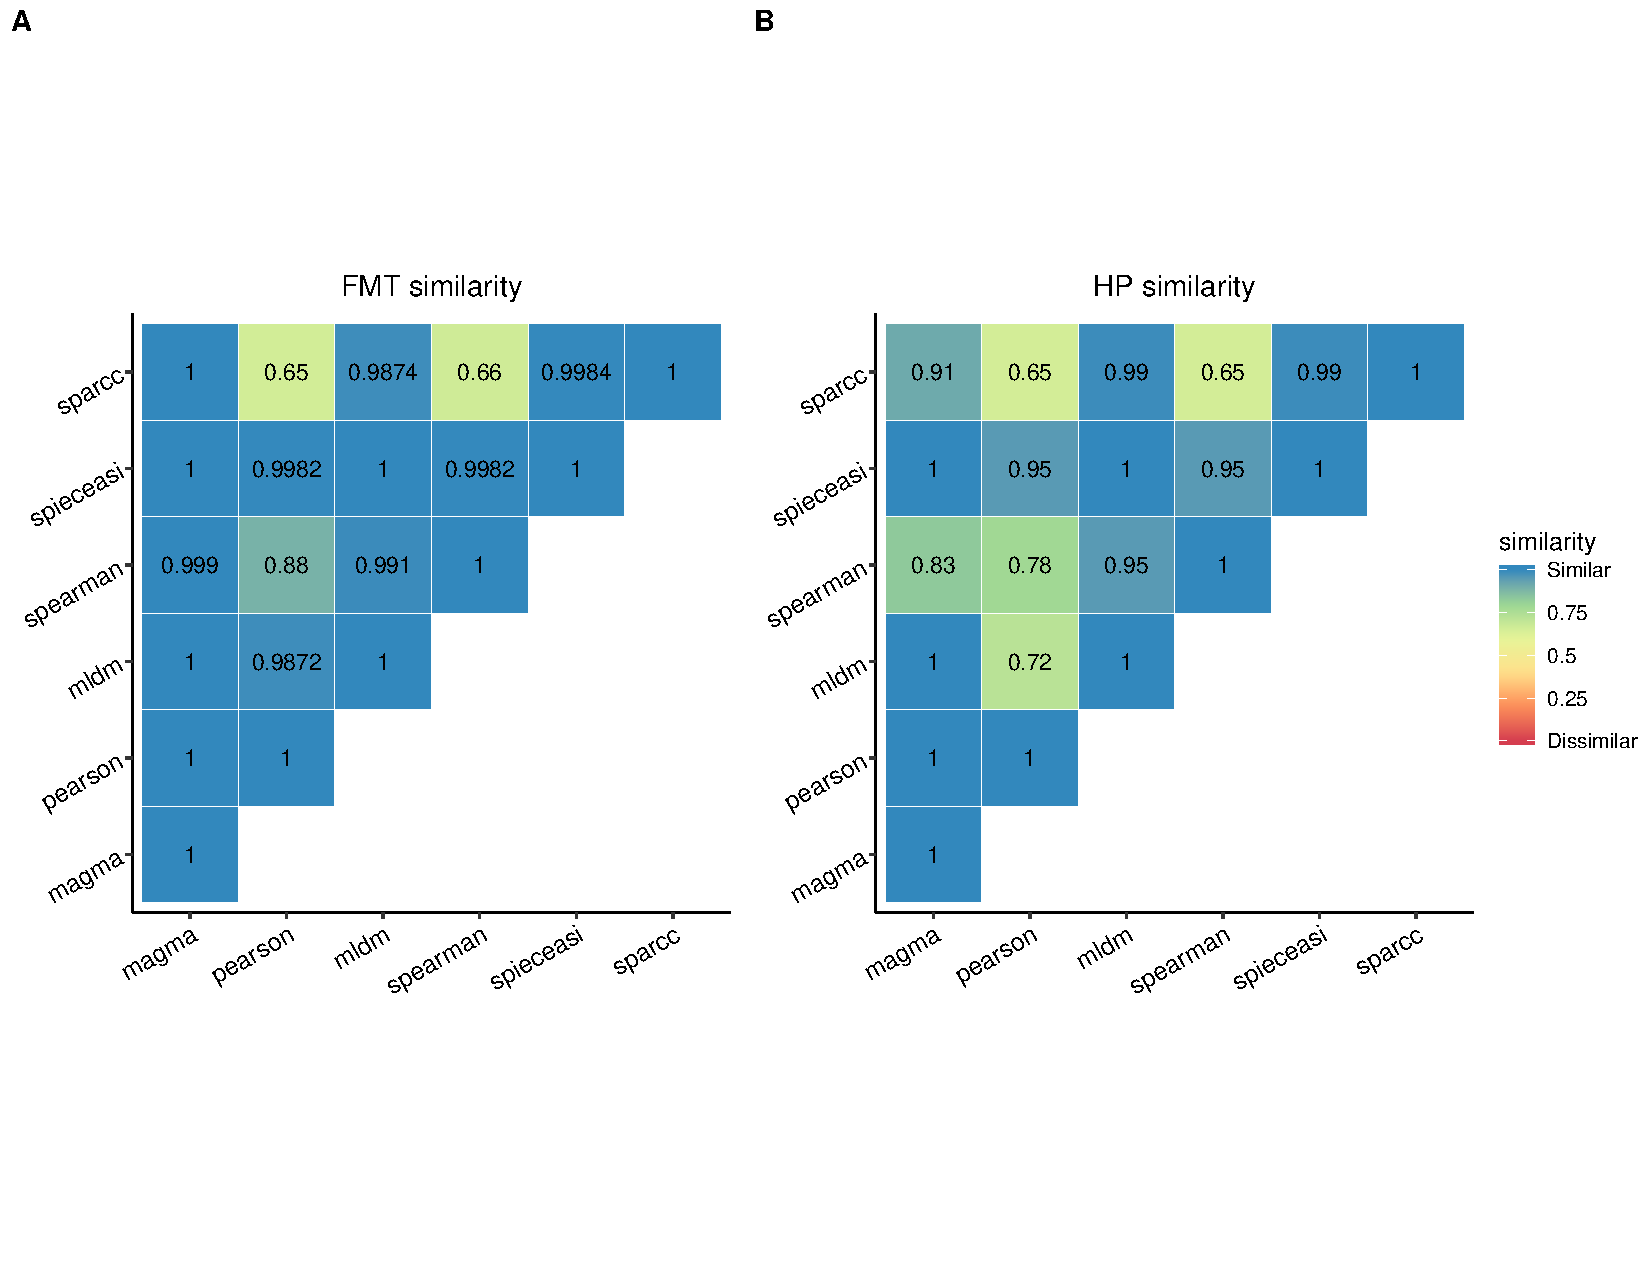
\includegraphics[width=\linewidth]{figureS8.pdf}
    \caption{
      The similarity between the networks generated using the different network inference algorithms for stool dataset (A) and the hard palate dataset (B).
      The similarity between the various methods was found to vary with the dataset used.
  }
    \label{fig:figureS8}
  \end{figure}

  \begin{figure}[h]
    \centering
    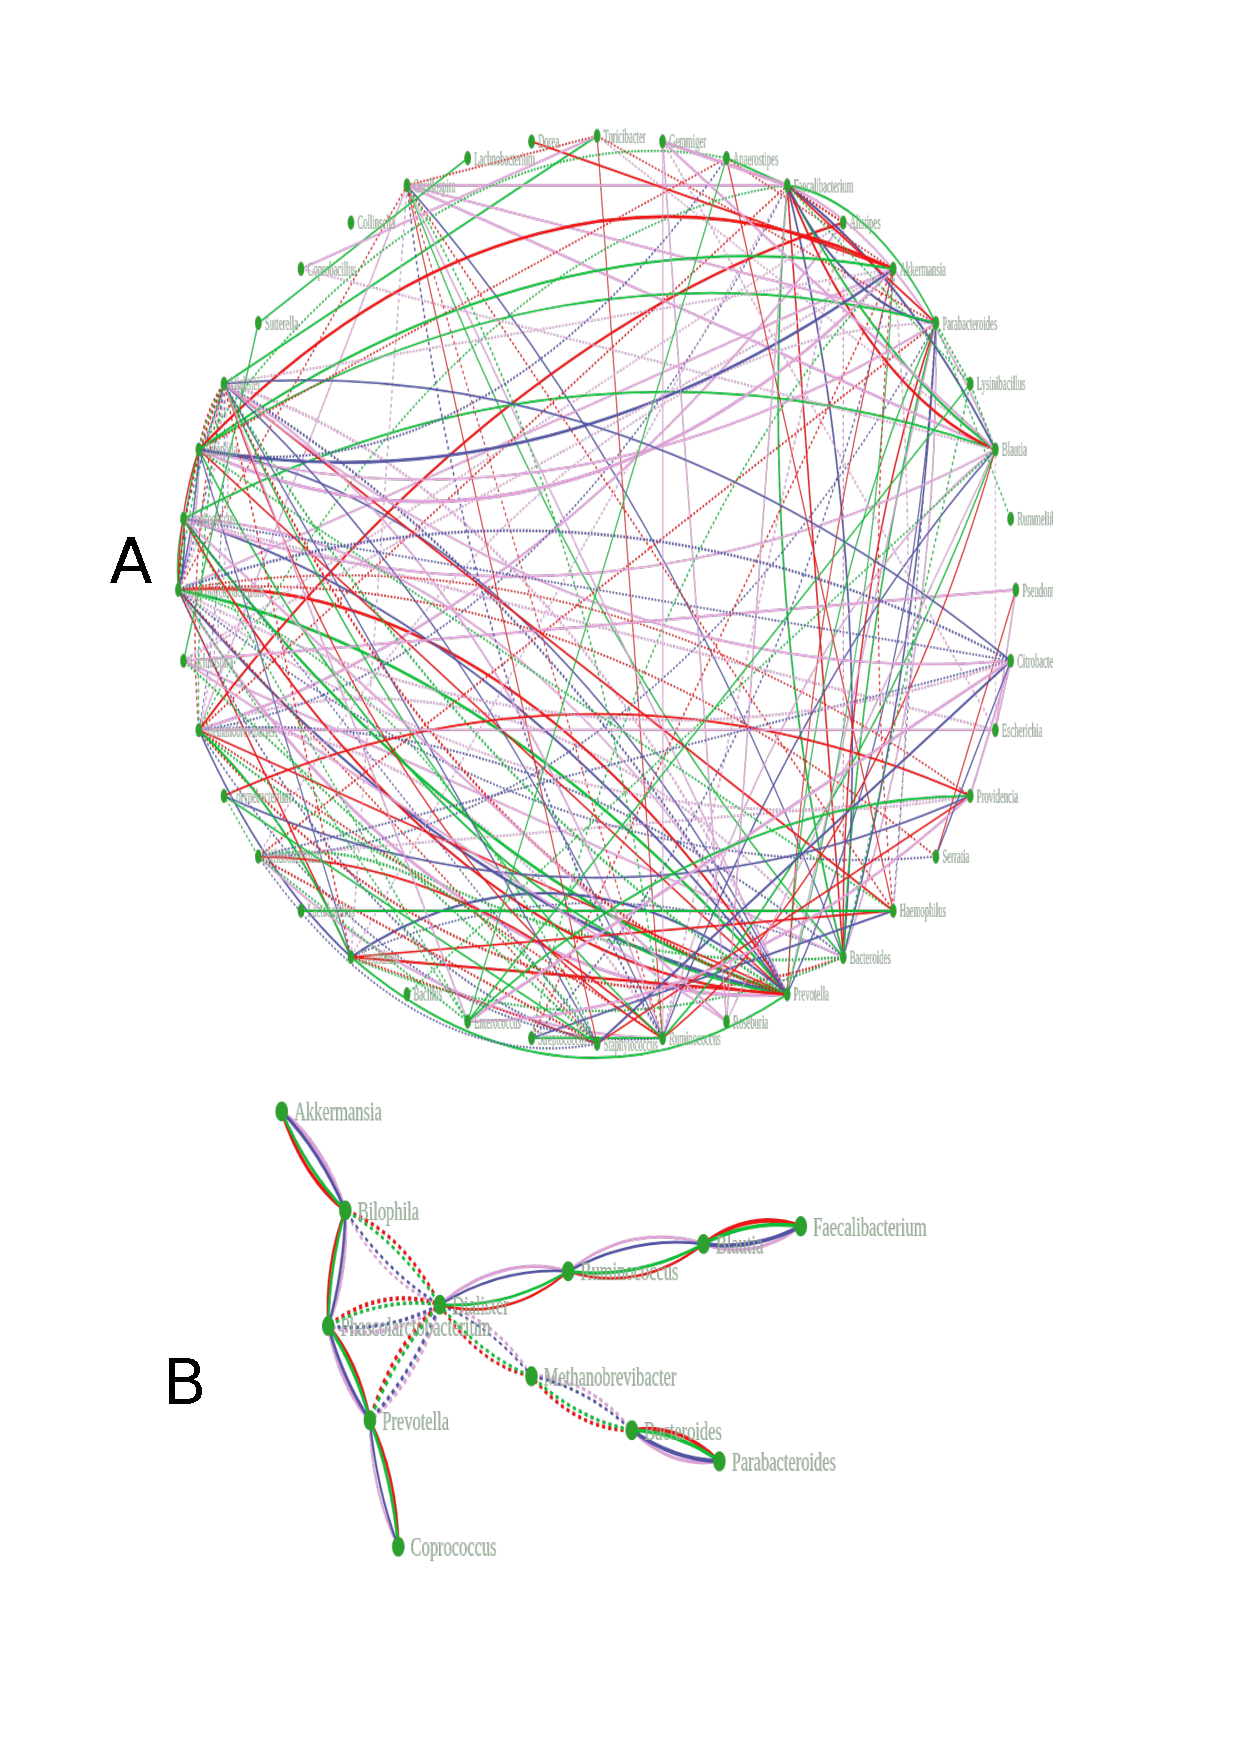
\includegraphics[width=0.8\linewidth]{pdf/denoise_network.pdf}
    \caption{A network showing union and intersection of networks generated using certain combination of methods}
    \label{fig:figureS5}
  \end{figure}
